\documentclass[letterpaper,openany,oneside,twocolumn]{book}

\usepackage[justified]{dnd}
\usepackage{ifthen}

\usepackage{dndtemplate}
\usepackage{bookmark}

\setlength\oddsidemargin{\dimexpr(\paperwidth-\textwidth)/2 - 1in\relax}
\setlength\evensidemargin{\oddsidemargin}

% Headline
\CharacterName{Nimrielle}
\CharacterSurname{Needleswift}
\CharacterNickname{Nim}

% adds only main class and total level to prevent overflow
\Class{Rogue (4) / Ranger (1)}
\Background{\href{https://dnd.wizards.com/products/tabletop-games/rpg-products/scag}{Urban Bounty Hunter (SCAG)}}
\PlayerName{Sam}
\Race{Lightfoot Halfling}
\Alignment{Neutral}
\XP{Milestone}
\Level{5} % total character level

% -------------------------------
%% ABILITIES %%

% Ability scores
\StrengthScore{9}           % Rolled 4,2,2,3 = 9
\DexterityScore{20}         % Rolled 6,6,6,3 = 18 +2 (Halfling) = 20
\ConstitutionScore{16}      % Rolled 5,5,6,1 = 16
\IntelligenceScore{13}      % Rolled 5,5,3,2 = 13
\WisdomScore{18}            % Rolled 6,6,6,6 = 18
\CharismaScore{16}          % Rolled 6,5,4,1 = 15 + 1 (Halfling Lightfoot) = 16

% Ability Modifiers
% The base modifier for each ability is calculated automatically from the ability scores using the formula:
%   Modifier = floor((Score - 10)/2)
% You can add an offset for racial traits, magic items, feats or other effects.
\StrengthModifier{0}       % Base calculation, no offset
\DexterityModifier{0}      % Base calculation, no offset
\ConstitutionModifier{0}   % Base calculation, no offset
\IntelligenceModifier{0}   % Base calculation, no offset
\WisdomModifier{0}         % Base calculation, no offset
\CharismaModifier{0}       % Base calculation, no offset


% -------------------------------
%% SAVING THROWS %%

% Saving Throws Proficiencies
\SetStrengthProficiency{1} % From Ranger class
\SetDexterityProficiency{1} % From Rogue/Ranger class
\SetConstitutionProficiency{0}
\SetIntelligenceProficiency{1} % From Rogue class
\SetWisdomProficiency{0}
\SetCharismaProficiency{0}

% The base modifier for each ability is calculated automatically from the ability scores using the formula:
%   Saving throw value = Ability modifier + Proficiency Bonus (if proficient)
% You can add an offset for racial traits, magic items, feats or other effects.
\SetStrengthSavingThrowModifier{0}      % Base calculation, no offset
\SetDexteritySavingThrowModifier{0}     % Base calculation, no offset
\SetConstitutionSavingThrowModifier{0}  % Base calculation, no offset
\SetIntelligenceSavingThrowModifier{0}  % Base calculation, no offset
\SetWisdomSavingThrowModifier{0}        % Base calculation, no offset
\SetCharismaSavingThrowModifier{0}      % Base calculation, no offset


% -------------------------------
%% SKILLS %%
% Skills Proficiencies
\SetAcrobaticsProficiency{1}            % From Rogue initial class      
\SetAnimalHandlingProficiency{0}
\SetArcanaProficiency{0}
\SetAthleticsProficiency{0}
\SetDeceptionProficiency{1}             % From Urban Bounty Hunter 
\SetHistoryProficiency{0}
\SetInsightProficiency{0}
\SetIntimidationProficiency{0}
\SetInvestigationProficiency{1}         % From Rogue initial class
\SetMedicineProficiency{0}
\SetNatureProficiency{2}                % Expertise from rogue archetype Scout
\SetPerceptionProficiency{2}            % From Ranger multi class, expertise from Ranger-Deft Explorer-Canny
\SetPerformanceProficiency{0}
\SetPersuasionProficiency{1}            % From Urban Bounty Hunter
\SetReligionProficiency{0}
\SetSleightOfHandProficiency{1}         % From Rogue initial class
\SetStealthProficiency{2}               % From Rogue initial class - Expertise from rogue lv1
\SetSurvivalProficiency{2}              % Expertise from rogue archetype Scout

% The base modifier for each ability is calculated automatically from the ability scores using the formula:
%  Skill value = Ability modifier + Proficiency Bonus (if proficient)
% You can add an offset for racial traits, magic items, feats or other effects.
\SetAcrobaticsSkillModifier{0}          % Base calculation, no offset
\SetAnimalHandlingSkillModifier{0}      % Base calculation, no offset
\SetArcanaSkillModifier{0}              % Base calculation, no offset
\SetAthleticsSkillModifier{0}           % Base calculation, no offset
\SetDeceptionSkillModifier{0}           % Base calculation, no offset
\SetHistorySkillModifier{0}             % Base calculation, no offset
\SetInsightSkillModifier{0}             % Base calculation, no offset
\SetIntimidationSkillModifier{0}        % Base calculation, no offset
\SetInvestigationSkillModifier{0}       % Base calculation, no offset
\SetMedicineSkillModifier{0}            % Base calculation, no offset
\SetNatureSkillModifier{0}              % Base calculation, no offset
\SetPerceptionSkillModifier{0}          % Base calculation, no offset
\SetPerformanceSkillModifier{0}         % Base calculation, no offset
\SetPersuasionSkillModifier{0}          % Base calculation, no offset
\SetReligionSkillModifier{0}            % Base calculation, no offset
\SetSleightOfHandSkillModifier{0}       % Base calculation, no offset
\SetStealthSkillModifier{0}             % Base calculation, no offset
\SetSurvivalSkillModifier{0}            % Base calculation, no offset


\Inspiration{}
\Perception{\fpeval{10+\PerceptionSkillModifierValue}}

\ArmorClass{
    \fpeval{
        11+ % Base AC for Leather Armor
        \DexterityModifierValue
    }
}
\Initiative{\DexterityModifierValue}
\Speed{\parbox{40pt}{\centering 7.5~m

\small{(4.5~swim)}}}
\MaxHitPoints{    \fpeval{
        8+ % Rogue first level
        8+ % Rolled at rogue level 2
        7+ % Rolled at rogue level 3
        3+ % Rolled at rogue level 4
        6+ % Default increase at ranger level 1
        \ConstitutionModifierValue * \LevelValue % Total levels
    }
}


\MaxHitDice{4d6+1d10}   % 4 from rogue, 1 from ranger
\CurrentHitDice{\LevelValue}

\CP{}
\SP{}
\GP{12} % 20 from Urban Bounty Hunter background, -8 for mule
\EP{}
\PP{}

% p = piercing, s = slashing, b = bludgeoning, 
\AddWeapon{Shortbow}{\fpeval{\ProficiencyValue+\DexterityModifierValue}}{1d6+
\DexterityModifierValue~/ % Because ranged weapon has dex modifier to damage
(x/96)-% Short bow has range 24/96 m, beyond 24 m you have disadvantage (my char has no disadvantage because has sharpshooter feat), you can not shoot beyond 96 m
p
}
\AddWeapon{Rapier}{\fpeval{\ProficiencyValue+\DexterityModifierValue}}{1d8+
\DexterityModifierValue~/ % Because finesse weapon has dex modifier to damage
p}
\AddWeapon{Dagger}{\fpeval{\ProficiencyValue+\DexterityModifierValue}}{d4+
\DexterityModifierValue~/ % Because finesse weapon has dex modifier to damage
(x/18)-% Dagger has range 6/18 m, beyond 6 m you have disadvantage (my char has no disadvantage because has sharpshooter feat), you can not throw beyond 18 m
p}


% \AttacksAdditional{
% \textbf{Guiding Bolt}: att. +4, dmg 4d6/r
% }

\OtherProficienciesLanguages{\textbf{Languages:} Halfling, Common, Orchish, % From Halfling + Background
Ogrish, Goblin. \\ % From Ranger-Deft Explorer-Canny + Background
\textbf{Weapons}: Simple weapons, hand crossbows, longswords, rapiers, shortswords, % From Rogue class
simple weapons, martial weapons.\\ % From Ranger class
\textbf{Armor}: Light Armor, % From Rogue Class
medium armor, shields.\\ % From Ranger class
\textbf{Tools}: Thieves' Tools (Expertise), % From rogue class, expertise from rogue lv1
Dragonchess set, % From Urban Bounty Hunter background
Musical instrument. % From Urban Bounty Hunter background
\\
}


\Equipment{
\textbf{Weapons}: \EquipmentItem{Rapier}{1}{1}, % From Rogue class
\EquipmentItem{Shortbow}{1}{1} + \EquipmentItem{Arrows}{0.025}{20}, % From Rogue class
\EquipmentItem{Dagger}{0.5}{2}.\\% From Rogue class
\textbf{Armor}: \EquipmentItem{Leather Armor}{5}{1}\\ % From Rogue class
\textbf{Tools}: \EquipmentItem{Thieves' Tools}{0.5}{1}\\ % From Rogue class
\textbf{Mounts/Animals}: Mule\\
\textbf{Misc}: \EquipmentItem{Traveler Clothes}{2}{1}, % From Urban Bounty Hunter background
\EquipmentItem{Pouch}{0.5}{1}, % From Urban Bounty Hunter background
\EquipmentItem{Backpack}{2.5}{1}, % From Explorer's Pack
\EquipmentItem{Bedroll}{3.5}{1}, % From Explorer's Pack
\EquipmentItem{Mess kit}{0.5}{1}, % From Explorer's Pack
\EquipmentItem{Tinderbox}{0.5}{1}, % From Explorer's Pack
\EquipmentItem{Torches}{0.5}{10}, % From Explorer's Pack
\EquipmentItem{Rations}{1}{10}, % From Explorer's Pack
\EquipmentItem{Waterskin}{2.5}{1}, % From Explorer's Pack
\EquipmentItem{Hempen rope (15 m)}{5}{1}\\ % From Explorer's Pack
\\
\textbf{Weight:} \EquipmentTotalWeight\ kg \\
\textbf{Capacity:} \newcommand{\Capacity}{\fpeval{
    \StrengthScoreValue*3+ % Homebrew carrying capacity formula
    210 % From mule
}}\Capacity\ kg\\
\textbf{Residual capacity:} \fpeval{\Capacity - \EquipmentTotalWeight} kg
}



\PersonalityTraits{
    \begin{itemize}
        \item Quiet, observant, and detail-oriented.
        \item Patient, calculating, and strategic.
        \item Distrustful of strangers; loyal to trusted allies.
    \end{itemize}
}

\Ideals{
    \begin{itemize}
        \item Freedom: oppose oppression and slavery.
        \item Survival: adapt and overcome harsh realities.
        \item Pragmatic Justice: right wrongs, even by gray means.
    \end{itemize}
}

\Bonds{
    \begin{itemize}
        \item Loyal to the Amazons who saved and trained her.
        \item Guided by the memory of her parents.
        \item Protects innocents in chaos or war.
    \end{itemize}
}

\Flaws{
    \begin{itemize}
        \item Presence of \textbf{orcs triggers a PTSD-fueled combat trance}; she becomes reckless and focused entirely on their destruction.
        \item Manipulative and secretive.
    \end{itemize}
}


\FeaturesTraits{
% From Halfling race
\textbf{Nimble}\\
\textbf{Lucky}\\
\textbf{Brave}\\
\textbf{Natural stealthy}\\
\textbf{Ear to the Ground}\\
\textbf{Sneak Attack}\\
\textbf{Thieves' Cant}\\
\textbf{Cunning Action}\\
\textbf{Skirmisher}\\
\textbf{Steady Aim}\\
\textbf{Favored foe}\\
\textbf{Sharpshooter}
}

\AdditionalFeaturesAndTraits{
\textbf{Archetypes}:\\
Rogue-\href{https://dnd5e.wikidot.com/rogue:scout}{Scout}\\
Ranger-\\
% From Halfling race
\textbf{Nimble}-> You can move through the space of any creature that is of a size larger than yours.\\
\textbf{Lucky}-> When you roll a \textbf{1} on the d20 for an attack roll, ability check, or saving throw, you can \textbf{reroll} the die and must use the new roll.\\
\textbf{Brave}-> You have \textbf{advantage} on saving throws against being \textbf{frightened}.\\
\textbf{Natural stealthy}-> You can attempt to hide even when you are only \textbf{obscured} by a creature that is at least one size larger than you.\\
% Background Feature from Urban Bounty Hunter
\textbf{Ear to the Ground}-> you have a \textbf{contact} in any city you visit, a person who provides information about the people and places of the local area.\\
% Rogue class features
\textbf{Sneak Attack}-> \textbf{2d6} if advantage on attack or enemy within 1,5 m of ally.\\
\textbf{Thieves' Cant}-> Secret mix of dialect, jargon, and code that allows you to hide messages in seemingly normal conversation.\\
\textbf{Cunning Action}-> Bonus action to \textbf{Dash}, \textbf{Disengage} or \textbf{Hide}.\\ % From lv2
\textbf{Skirmisher}-> You can \textbf{move up to half your speed as a reaction} when an enemy ends its turn within 1,5 m of you without provoking opportunity attacks.\\ % From archetype Scout
\textbf{Steady Aim}-> On your turn, you can use a \textbf{bonus action} to give yourself \textbf{advantage} on your next attack roll on the current turn. You can use it if you \textbf{haven't moved} and \textbf{speed is 0} until end of turn.\\ % From lv3
% Ranger class features
\textbf{Favored foe}-> mark target for 1 minute or until lose concentration, on hit the target receives \textbf{1d4} extra damage. Can be used \textbf{\ProficiencyValue} times per longrest.\\
% Talents
\textbf{Sharpshooter}-> Attacks at long range don't impose disadvantage, ignore half and three-quarters cover, before attack you can choose to take \textbf{-5} to hit for \textbf{+10} damage.
}

% Appearance

\Age{28}
\Height{0.97 m}
\Weight{18 kg}
\Eyes{Grey-blue}
\Skin{Light tan}
\Hair{Blonde-red}

% background

\CharacterAppearance{
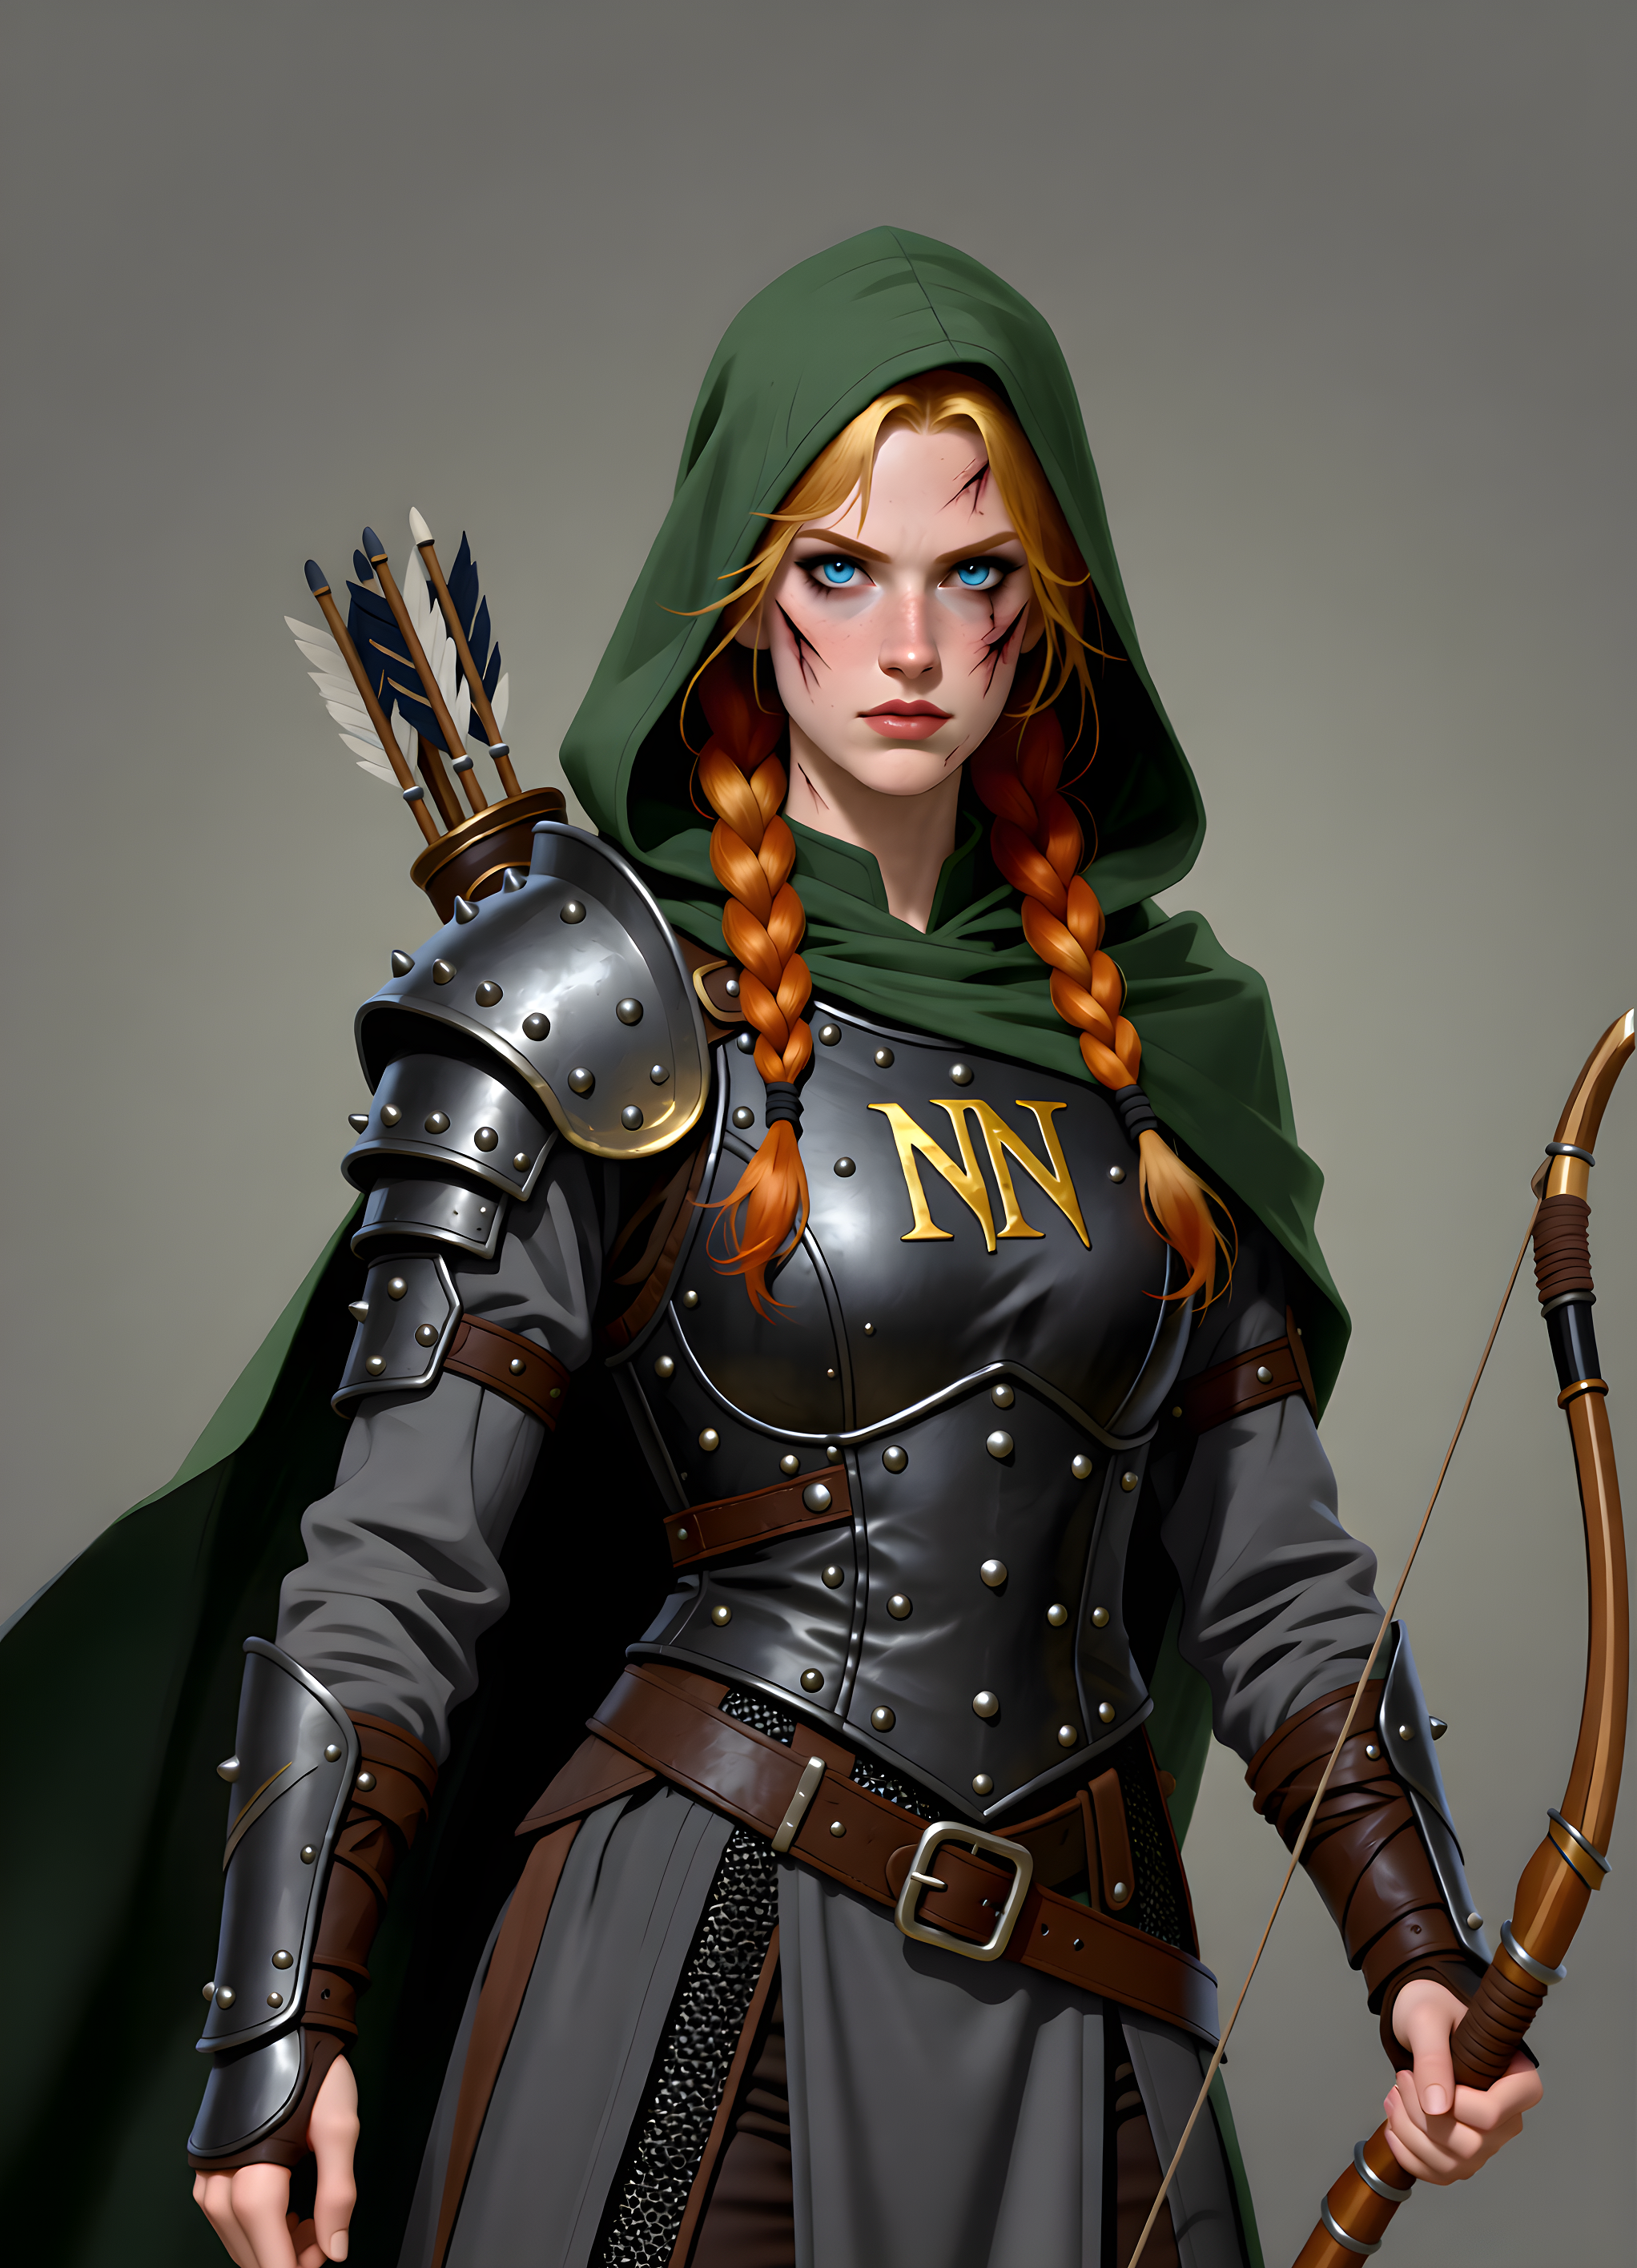
\includegraphics[width=5.7cm]{characters/images/nim.png}
}



\Characterbackground{
    Nimrielle Underbough, a halfling born in 1468 DR to a wandering merchant family along the High Road, grew up learning the arts of survival and subtlety from her parents. In 1485 DR, her life changed forever when Nightstone was attacked by a castle in the clouds, killing her mother and forcing her father to flee with her. The following year, she endured captivity by ogres, followed by slavery among the Orc clans in 1486-1488 DR, experiences that shaped her into a resourceful and cautious survivor, but deeply traumatized her.\\

    In 1488 DR, Nimrielle was rescued by the Amazons, a mercenary clan devoted to Tempus, who healed her body and mind and guided her through the Ierodule rites. Between 1491-1493 DR, she was trained as a shadow operative, honing his skills in stealth and infiltration. Her exceptional skill in reconnaissance and cunning earned her recognition and eventual early release from active service in 1493-1494 DR, after which she worked as a bounty hunter along the Sword Coast.\\

    By 1494-1496 DR, Nimrielle had carved out a life in the cities as a bounty hunter, when a mysterious letter commanded her to meet someone in Honeywood. 
 }

\Treasure{
}

\AlliesAndOrganizations{
    \begin{itemize}
        \item The Amazons: Mercenary clan and spiritual mentors who saved her from slavery.
        \item Former contacts from bounty hunting along the Sword Coast: informants, guides, and fences.
        \item Luna: A young Amazon recruit who admires Nimrielle and reminds her of a lost innocence.
    \end{itemize}
}

\OrganizationName{The Amazons
}
\OrganizationSymbol{\includegraphics[width=4.9cm,height=3.9cm]{characters/images/amazons-banner}
}


%Magic
\SpellcastingClass{}
\SpellcastingAbility{}
\SpellSaveDC{}
\SpellAttackBonus{}

\FirstLevelSpellSlotsTotal{}

\FirstLevelSpellSlotA{}
\FirstLevelSpellSlotAPrepared{}
\FirstLevelSpellSlotB{}
\FirstLevelSpellSlotBPrepared{}
\FirstLevelSpellSlotC{}
\FirstLevelSpellSlotCPrepared{}
\FirstLevelSpellSlotD{}
\FirstLevelSpellSlotDPrepared{}
\FirstLevelSpellSlotE{}
\FirstLevelSpellSlotEPrepared{}
\CantripSlotA{}
\CantripSlotB{}
\CantripSlotC{}
\CantripSlotD{}

\newcommand{\spellsheetchoice}{\renderspellsheet}


\usepackage{hyperref}
\hypersetup{ colorlinks=true }
\begin{document}
\newgeometry{left=0cm,right=0cm,top=0cm,bottom=0cm}
\onecolumn


% CHARACTER PAGE
\pdfbookmark[0]{Character Sheet}{Character Sheet}
\rendercharactersheet

% BACKSTORY PAGE
\pdfbookmark[0]{Background Sheet}{Background Sheet}
\renderbackgroundsheet


% SPELLCASTING PAGE
\pdfbookmark[0]{Spellcasting Sheet}{Spellcasting Sheet}
\spellsheetchoice

\newpage

\section{Full Character Background of \CharacterFullNameValue}
\subsection{1468-1484 DR — Childhood Along the High Road}
Nimrielle Needleswift was born in 1468 DR into a wandering halfling family of merchants. Her parents, Lira and Tobin Needleswift, had no permanent home; they followed the trade caravans that wound through the northern stretches of the Sword Coast, often pausing in the quiet village of Nightstone, where commerce and travelers were never in short supply.\\

Nimrielle's childhood was modest but filled with simple joys. Her father taught her to move silently, like a mouse threading through the forest underbrush, while her mother showed her how to read the signs of the wild—tracking animals, recognizing footprints, and identifying useful plants. There was no formal training, only the education of life along the road, but it gifted her with a keen instinct for survival.\\

Everything changed when Nimrielle turned seventeen.

\subsection{1485 DR — The Castle in the Clouds and Flight Toward Death}
The year 1485 brought an abrupt end to Nimrielle's childhood. One morning, as the sun crested over Nightstone, a castle appeared in the clouds above the village—a fortress of the cloud giants. From its lofty heights, enormous boulders rained down, smashing homes and crushing the marketplace. Panic tore through the streets.\\

Lira Needleswift, Nimrielle's mother, shielded her daughter from the falling stones. One struck too close—Lira's life ended in an instant, leaving Nimrielle trembling amidst the ruins. Her father, Tobin, dragged her from the wreckage, shouting for her to run. Together, they fled toward the hills north of Nightstone, where other survivors huddled in caves.\\

But safety was an illusion. The first weeks were mostly idle; the survivors tried to grasp the enormity of what had happened to them. Eventually, they ventured deeper into the caves, carving out a fragile semblance of life. For a time, it seemed they might endure, building shelters and finding a rhythm amidst the stone.\\

Then, months later, came the sound they would never forget—drums, echoing from the depths. And with the drums came the goblins. The creatures swarmed from shadowed tunnels, merciless and relentless. What followed was a nightmarish battle—chaotic, endless, with screams reverberating through the rock. One by one, the Nightstone fighter fell. Tobin with a group of non fighter was escorting a group of children and women toward safety. but soon the goblin were after them. When an arrow struck him in the back Nimrielle did not look back and started running for her life. She ran as fast as her legs could carry her, leaving the caves behind, barely a handful of survivors escaping with her.

\subsection{1486 DR — The Ogre Captivity}
Grief-stricken and utterly exhausted, Nimrielle ran without direction. Her thoughts were a blur, her heart heavy with the loss of her parents and the horrors she had witnessed. Rather than seeking the scattered human settlements to the north, her feet carried her deeper into the jagged hills, where shadows lengthened and caves yawned like hungry mouths. She stumbled into a narrow ravine, hoping for shelter, only to freeze at the echo of low, guttural laughter.\\

From the darkness, two massive figures emerged—ogres, towering and grotesque, their cruel eyes glinting with morbid amusement. Nimrielle tried to flee, but her limbs betrayed her; exhaustion and despair had sapped every ounce of strength. A massive hand clamped down on her shoulder, lifting her with terrifying ease.\\

The ogres, amused by the tiny human, decided to keep her—not as a prisoner to torment, but as a strange, living companion. They named her “little one” in their rough tongue, and though she was treated like a pet, they showed a certain decency: they shared their food, allowed her to walk beside them, and even spared her from the rougher whims of ogre society. In their crude, brutal way, they preserved her life.\\

Months passed as they roamed north, eventually reaching the Nebldarpèrng region. There, high among jagged cliffs, lay Schmugenrock—an ancient dwarven village abandoned for centuries. Its name had been seized by the black dragon Schmug, who had ruled the settlement for ages before gifting it to the Many-Arrows Orc clan for their loyalty.\\

The Many-Arrows had recently been fractured by civil war, and the traditionalist faction now roamed the High Road, raiding any caravan or traveler that dared pass. As the ogres passed through the cliffs, they were ambushed by a band of these orcs. The confrontation quickly escalated; a violent skirmish erupted. Outnumbered, the ogres fought fiercely but were ultimately overwhelmed. Nimrielle was captured by the orcs.

\subsection{1486-1488 DR — Slavery Among the Orcs and the Birth of the Thief}
For two long years, Nimrielle's existence became a living nightmare.\\

Gurthak Jawsplitter, the brutal leader of the orc band that had captured her, spared her life—but not out of mercy. She was valuable to the clan as a plaything, and in their cruel eyes, that meant subjugation. Nimrielle was forced into sexual servitude, her days and nights marked by torment, humiliation, and relentless hunger. She learned to scavenge scraps of food from her captors just to survive. Not every attempt succeeded, and failure brought punishments designed to break both body and spirit: sometimes she was forced to eat beside the clan's animals, at other times compelled to consume filth—or even the remains of unfortunate victims from the orcs' raids. Pain, degradation, and fear became her constant companions.\\

Yet, even amid suffering, Nimrielle survived—and in surviving, she learned to thrive in the shadows. Necessity honed her into a natural thief. She became a master of stealth, moving silently through darkness so as not to alert the towering orcs. She watched, memorized, and anticipated their routines, learning when and where danger would strike. She improvised tools to lift locks or manipulate objects, assessed risks in an instant, and plotted escape routes with meticulous care. Everytime she tried to escape she was caught and further brutalized, but each failure only strengthened her will to escape.\\
During these terrible years of imprisonmentcaptivity, Nimrielle's hatred for the orcs grew into something almost tangible, a visceral hate that burned her from the inside. She reached the conclusion that the only way to survive was to understand her captors deeply. She learned their language, studied the clan's behaviors, hierarchies, and gestures. 

\subsection{1488-1491 DR — The Amazons and the Rebirth}
But in 1488 DR, a miracle intervened.\\

The orcs of Gurthak Jawsplitter, fueled by their unchecked raids and arrogance, set upon a caravan traveling the High Road near Tunkhlbalt, a bustling city under the watchful eye of the Amazon Clan, defended by their renowned mercenary army.\\

As the orcs launched their attack, the mercenary cavalry appeared over a nearby hill. The battle was swift and merciless—disciplined steel and divine fury guided the Amazons’ blades, cutting down orcs where they stood. Those who fled led the scouts back to the rest of the party, only to meet the same fate. Amid the slaughter, Nimrielle was found, chained, battered, and broken in spirit.\\

According to the traditions of the Clan, a freed slave was not simply liberated. She became an Ierodule of the Temple: not a servant in bondage, but a sacred acolyte, woven into the rituals of Tempus and Ishtar. Carried into the holy district, Nimrielle was tended, fed and healed. The transition from torment to sanctity was strange and at times agonizing, yet it marked the beginning of her true rebirth.\\

During the years as an Ierodule, Nimrielle learned to distinguish cruelty from reverence. She was free to refuse sacre service, free to rest, free to exist as a person rather than an object. It was during this time that the Amazons began to notice peculiar traits: Nimrielle moved without a sound and she could vanish into shadows without even trying. By the end of her Ierodule training, the Clan recognized her potential and was evaluated as a prospective recruit for the Amazon mercenary company.

\subsection{1491-1493 DR — The Training of a shadow}
By 1491 DR, at the age of twenty-four, Nimrielle left behind the sacred duties of the \textit{Ierodule} to step into a new life of discipline within the Amazon Clan's ranks.\\
The Amazons saw in her an uncanny gift. When she took up a bow, accuracy was not merely a matter of skill—she decided where her arrow would land. Her shots bent around wind, distance, and timing as though the world quietly adjusted itself to her will. It was a talent as unsettling as it was impressive, and the instructors swiftly realized they were shaping a true sharpshooter. Under their guidance, she mastered the art of ranged combat.\\
But raw talent was only the foundation.\\
What set Nimrielle apart were the instincts instilled in her by her mother during her childhood wandering the High Road. Her mother tought her how to read a footprint, how to sense a presence in the brush, how to disappear into the quiet of a forest.\\

Her training was relentless. Days bled into nights and back again as she learned to:
\begin{itemize}
    \item she could infiltrate enemy lines unseen;
    \item deliver silent, lethal eliminations;
    \item gather secrets without leaving a trace;
    \item strike from shadows with deadly accuracy;
    \item move with the swiftness of a startled deer, delivering decisive blows before an enemy could react.
\end{itemize}
By the end of this training, Nimrielle was a scout of unparalleled skill.

\subsubsection{The Girl Who Watched Her Train}
Luna started showing up at the training grounds. Like the other younger recruits, she was curious about the halfling shadow. Nimrielle noticed her quickly—the girl always stood in the same place, watching with a focus far stronger than the others. Thirteen years old, maybe, Amazon-born from her posture alone.\\

Nimrielle ignored her at first. She had drills to survive and instructors who didn't care if she bled or collapsed due to exhaustion. But Luna kept coming back, tracking every movement Nimrielle made: how she stepped, how she drew her bow, how she slipped behind a post and appeared on the other side. One evening, Nimrielle caught her behind a tent trying to copy her footsteps. Luna froze, expecting a reprimand. Nimrielle just gave a brief nod and showed her the movement—not with much success, but she tried.\\

After that, Luna stayed closer. And as the weeks went by, Nimrielle found herself growing unexpectedly fond of the girl. Luna reminded her of a time before everything had been taken from her—a time when she'd been young, and innocent, and unaware of how cruel the world could be. Being around Luna brought a small piece of that back.


\subsection{1493-1494 DR — A Dirty Business}
The Amazons granted a warrior the right to leave the mercenary company after ten years of service—or sooner, if their deeds were truly extraordinary. Nimrielle, however, had learned early that courage alone could not guarantee survival in a world as brutal and unpredictable as hers. She understood that cunning, subtlety, and the ability to manipulate events from the shadows were often more valuable than brute force.\\

Her opportunity arrived during a mission that would change the trajectory of her life. The task demanded infiltration, intelligence gathering, and complete invisibility within a hostile settlement. The target was Klebostuo, a goblin stronghold perched along a jagged pass. Nimrielle’s small, nimble frame allowed her to slip unnoticed among the goblins, and her natural agility made her the ideal scout. Even more, her knowledge of Orcish accelerated her learning of Goblin, allowing her to eavesdrop, communicate, and interpret enemy movements without raising suspicion.\\

For months, she moved like a shadow, observing goblin patrols, noting their schedules, mapping hidden passages, and discovering weak points in the fortress defenses. She infiltrated their storage areas, subtly sabotaged supply chains, and silently relayed critical intelligence back to her superiors. Her work was methodical, patient, and precise; a single misstep could have meant death, yet she thrived in the chaos that others would have feared.\\

One operation nearly went awry. A reckless, arrogant warrior named Rhyssara had always dismissed Nimrielle’s skill, treating her with thinly veiled contempt. When a mission objective was on the brink of failure, Nimrielle recognized an opportunity. She carefully manipulated the circumstances so that Rhyssara appeared responsible for the mishap, drawing suspicion and leaving her rival vulnerable to goblin retaliation. Simultaneously, Nimrielle corrected the situation, completing the mission flawlessly and ensuring the outcome aligned with her version of events.\\

Her exceptional performance did not go unnoticed. The Amazons were impressed not just by her skill, but by her ingenuity in turning the mission from a potential disaster into a triumph. As a result, Nimrielle earned an early discharge from daily active service. She was free to roam as she wished, no longer bound to the regimented duties of the mercenary company. Yet her talents remained too valuable to ignore entirely. The Amazons knew that when the stakes were highest, when cunning and precision were required in equal measure, Nimrielle would be summoned.

\subsection{1494-1496 DR — The Letter}
By now, Nimrielle—known to most simply as “Nim”—had carved out a quiet, precarious life as an urban bounty hunter. She roamed the streets of the Sword Coast cities, tracking bounties for money, always employing the tactics learned during her training days.\\

One bleak winter morning, a letter arrived, slipped silently under the door of her modest lodgings. It was folded with meticulous care, unsealed, and written in the perfect, angular script of someone highly trained in the art of writing. There was no signature, no flourish, only a message so brief it seemed almost polite—if not for the veiled menace it carried. It read:
\begin{quote}
   \textit{Nimrielle Needleswift.}\\
    \textit{I know how you won your freedom.}\\
    \textit{I know whom you betrayed.}\\
    \textit{Present yourself to the Hag's Baron in Honeywood, at dawn on the 5th of Alturiak.}\\
    \textit{Come alone.}
\end{quote}
Nim's stomach tightened. No one knows her by her full name \textit{Nimrielle Needleswift} only the Amazons remembered it fully. She read the words again, and a chill unlike any winter frost crept down her spine. It was not merely the cold of the North Sword Coast that struck her—it was the terror of knowing that \textit{Someone} knew. And that \textit{Someone} now demanded her presence.\\

After several days of travel, Nim arrived in Honeywood. She contacted her local informant, hoping for information about the town and any clue as to who might have sent the letter, but they had no relevant information. She also watched the area around the tavern from a discreet distance, but found nothing of note.\\

When the time of the convocation came, Nim stood outside the inn, her cloak wrapped tightly against the biting wind, her hand resting lightly on the hilt of her dagger. She was not ready to enter, yet with a deep breath, she stepped across the threshold and ventured inside.

\end{document}
